\documentclass[
	12pt,				% tamanho da fonte
	openright,			% capítulos começam em pág ímpar (insere página vazia caso preciso)
	oneside,			% para impressão em verso e anverso. Oposto a oneside
	a4paper,			% tamanho do papel. 
	english,			% idioma adicional para hifenização
	french,				% idioma adicional para hifenização
	spanish,			% idioma adicional para hifenização
	brazil				% o último idioma é o principal do documento
	]{abntex2}

% Pacotes essenciais
\usepackage[utf8]{inputenc}
\usepackage[T1]{fontenc}
\usepackage[brazil]{babel}           % Hifenização e datas em português
\usepackage{amsmath}
\usepackage{amsfonts}
\usepackage{amssymb}
\usepackage{graphicx}
\usepackage{indentfirst}
\usepackage{xurl}                    % Substitui url e breakurl
\usepackage{float}
\usepackage{caption}
\usepackage{subcaption}
\usepackage{longtable}
\usepackage{booktabs}
\usepackage{multirow}
\usepackage{array}
\usepackage{enumitem}
\usepackage{soul}
\usepackage{xcolor}
\usepackage[alf]{abntex2cite}
\newcommand{\citet}[1]{\citeauthoronline{#1} (\citeyear{#1})}


% hyperref já é carregado pelo abntex2; usar \hypersetup para opções adicionais
\usepackage{hyperref}
\hypersetup{breaklinks=true}
\setlength{\emergencystretch}{3em}

\graphicspath{{images/}}

% Suprime erro de \theforeigntitle no \maketitle do abntex2 article
\providecommand{\theforeigntitle}{}

% Reduz espaço após títulos de capítulo e seção (memoir nativo)
\setlength{\beforechapskip}{0pt}
\setlength{\afterchapskip}{1em}


% Informações do documento
\title{Desempenho Educacional nos Municípios Maranhenses: Uma Análise Comparativa entre as Regiões do Estado}
\author{Darlon José Coqueiro}
\date{\today}

\begin{document}

\vspace*{-2cm}
\begin{center}
  
\includegraphics[scale=0.5]{images/logo_ifma.png}\\[1cm]
  {\large\bfseries Desempenho Educacional nos Municípios Maranhenses: Uma Análise Comparativa entre as Regiões do Estado}\\[0.5cm]
  {\normalsize Darlon José Coqueiro}\\[0.3cm]
  {\normalsize \today}
\end{center}
\vspace{2em}
\pagestyle{plain}


\section*{Resumo}

\noindent
Esta investigação analisa o desempenho educacional no IDEB EFAI 2023 (Índice de Desenvolvimento da Educação Básica, Anos Iniciais do Ensino Fundamental) das escolas da rede municipal, utilizando aprendizado de máquina não supervisionado para identificar padrões associados ao desempenho escolar em contextos de vulnerabilidade socioeconômica. Integrando microdados do Censo Escolar 2023 e indicadores socioeconômicos do IBGE para os 217 municípios do estado com dados disponíveis, adotamos uma abordagem em dois estágios: segmentação municipal via \textit{K-Means} sobre renda \textit{per capita} e IDHM (Índice de Desenvolvimento Humano Municipal), seguida de \textit{Random Forest Classifier} e testes de Mann-Whitney para identificar, dentro de cada grupo, os fatores que diferenciam municípios de alto e baixo desempenho no IDEB. Os resultados identificaram os fatores mais fortemente associados ao desempenho superior. Essas descobertas evidenciam a utilidade do aprendizado não supervisionado para análises educacionais descritivas e oferecem subsídios concretos para políticas educacionais e de alocação de recursos nos municípios. Esta pesquisa contribui para suprir a sub-representação do Maranhão na literatura de mineração de dados educacionais e propõe uma estrutura analítica replicável para outras regiões em desenvolvimento que busquem orientar estratégias de educação pública a partir de dados administrativos.

\medskip
\noindent\textbf{Palavras-chave:} desempenho educacional; IDEB; IDHM; municípios maranhenses; clusterização; \textit{K-Means}; \textit{Random Forest}; políticas educacionais.
\chapter{Introdução} \label{cap:intro}

A qualidade da educação básica é um dos principais determinantes do desenvolvimento humano e econômico de longo prazo \cite{hanushek2012}. No Brasil, o Índice de Desenvolvimento da Educação Básica (IDEB) monitora o ensino público combinando fluxo escolar e proficiência em língua portuguesa e matemática numa medida comparável entre municípios, estados e redes de ensino \cite{fernandes2007}. Apesar dos avanços das últimas duas décadas, as disparidades regionais persistem: estados do Norte e do Nordeste ficam sistematicamente abaixo da média nacional, reflexo de desigualdades estruturais de renda, infraestrutura e serviços públicos \cite{inep2023}.

O Maranhão está entre os casos mais críticos. Com um dos menores IDHMs do país e indicadores educacionais historicamente abaixo da média nacional, o estado concentra municípios em alta vulnerabilidade socioeconômica, onde os obstáculos para melhorar o desempenho escolar superam a capacidade de gestão local \cite{ibge2010, inep2023}. Isso coloca uma pergunta direta: o que diferencia, dentro de um mesmo patamar de vulnerabilidade, os municípios que sobem no IDEB daqueles que ficam estagnados?

A literatura internacional examinou amplamente a relação entre condições socioeconômicas, infraestrutura escolar, qualificação docente e o desempenho dos estudantes \cite{rivkin2005, coleman1966}. No Brasil, estudos com dados do IDEB e do Censo Escolar apontaram formação dos professores, tamanho das turmas e infraestrutura como variáveis relevantes \cite{vasconcelos2021, soares2013}. Análises voltadas especificamente para o Maranhão que isolem fatores intracontextuais (aqueles que operam mesmo quando o contexto socioeconômico é semelhante) são escassas.

Métodos de aprendizado de máquina têm sido aplicados a dados educacionais com resultados promissores, especialmente por sua capacidade de lidar com bases administrativas grandes e heterogêneas \cite{baker2010, romero2020}. Algoritmos de agrupamento identificam estruturas nos dados sem categorias predefinidas, o que os torna úteis para segmentar contextos antes de comparações \cite{faceli2021}. Quando combinados com medidas de importância de variáveis e testes não paramétricos, essa abordagem permite identificar os fatores que mais diferenciam grupos de desempenho.

Este trabalho aplica essa lógica aos 217 municípios maranhenses com dados disponíveis no IDEB 2023 (Anos Iniciais do Ensino Fundamental, rede municipal). No primeiro estágio, os municípios são agrupados por contexto socioeconômico via K-Means, usando renda per capita e IDHM. No segundo, dentro de cada grupo, um Random Forest Classifier combinado com o teste de Mann-Whitney identifica quais características escolares e socioeconômicas separam municípios de alto e baixo desempenho. As variáveis analisadas vêm do Censo Escolar 2023: infraestrutura (internet, biblioteca, laboratório de informática, saneamento), qualificação docente e indicadores de fluxo escolar.

O trabalho faz três contribuições principais. Primeiro, propõe e aplica ao contexto específico do Maranhão uma abordagem em dois estágios (segmentação socioeconômica seguida de análise intragrupo). Segundo, identifica os fatores escolares associados ao desempenho superior no IDEB entre municípios vulneráveis. Terceiro, disponibiliza um pipeline reprodutível para análises similares em outras unidades federativas. Os resultados têm uso direto para gestores e formuladores de políticas que precisam decidir onde concentrar recursos.

O restante do artigo está organizado da seguinte forma: o Capítulo~\ref{cap:related} apresenta os trabalhos relacionados; o Capítulo~\ref{cap:methods} descreve os materiais e métodos; o Capítulo~\ref{cap:experiments} apresenta os experimentos e resultados; o Capítulo~\ref{cap:conclusions} discute conclusões, limitações e direções futuras.
\chapter{Related Works}
\label{cap:related}

\section{Supervised Machine Learning in Educational Analytics}

\section{Unsupervised Learning for Pattern Discovery}

\section{IDEB-Based Studies and Socioeconomic Factors}

\section{Our Proposal}
\chapter{Material and Methods}
\label{cap:methods}

\section{Machine Learning}


\section{Association Rules}


\section{Methodology}

\chapter{Experimentos Computacionais}
\label{cap:experiments}

\section{Compreensão do Domínio}

O Maranhão é o segundo maior estado do Nordeste em extensão territorial e um dos mais populosos, com 217 municípios distribuídos em cinco mesorregiões. Em indicadores socioeconômicos, ocupa posições críticas: IDHM médio de 0,639 em 2010 (um dos mais baixos do país) e renda per capita municipal mediana em torno de R\$~200 no mesmo período \cite{ibge2010}. Esse contexto reflete-se diretamente nos resultados educacionais: na edição 2023 do IDEB, a média dos municípios maranhenses nos Anos Iniciais da rede municipal ficou em 5,01, com metade dos municípios abaixo de 4,90, valores que evidenciam tanto o atraso histórico quanto a dispersão expressiva do desempenho entre municípios.

A questão central desta investigação é identificar, entre municípios com contexto socioeconômico semelhante, quais fatores escolares estão associados ao desempenho superior no IDEB. Respondê-la exige, primeiro, neutralizar o efeito do contexto por meio de uma segmentação explícita e, depois, comparar, dentro de cada grupo, os municípios de alto e baixo desempenho.

\section{Coleta de Dados}

O pipeline de ingestão (\texttt{ingest.py}) automatiza a carga das quatro fontes descritas no Capítulo~\ref{cap:methods}. Para o IDEB, lê a planilha oficial do INEP e filtra os municípios maranhenses da rede municipal, tratando os códigos de não divulgação (ND, ND*, (*), (**)) como valores ausentes. Para o Censo Escolar, carrega os microdados em formato CSV (encoding latin-1, separador ponto-e-vírgula) e seleciona as colunas de infraestrutura, docentes e matrículas, filtrando as escolas de dependência municipal no Maranhão (TP\_DEPENDENCIA = 3). Para os docentes dos Anos Iniciais, usa exclusivamente a Tabela 2.23 da Sinopse Estatística 2023 (formato ODS), garantindo que numerador (docentes com superior) e denominador (total de docentes EFAI) venham da mesma fonte. O IBGE e o IDHM são lidos de planilhas Excel curadas previamente.

As variáveis de infraestrutura são agregadas ao nível municipal como proporção de escolas com cada atributo presente. As variáveis de docentes, como percentual sobre o total de docentes EFAI do município. As variáveis de fluxo, como médias ou proporções sobre o total de matrículas e turmas municipais.

\section{Pré-processamento}

O pipeline de transformação (\texttt{transform.py}) aplica as seguintes operações:

\begin{itemize}
  \item \textbf{IDEB:} substituição de valores especiais por \texttt{NaN}, conversão de vírgula para ponto decimal, remoção de colunas redundantes (notas separadas de LP e MAT, já incorporadas na nota média).
  \item \textbf{Censo Escolar:} remoção de colunas completamente vazias, conversão de colunas de quantidade para inteiro, normalização do código municipal para 7 dígitos.
  \item \textbf{IBGE:} remoção de linhas de totalização regional, normalização de nome de colunas.
  \item \textbf{IDHM:} remoção de linhas de totalização, renomeação de colunas para padrão interno.
  \item \textbf{Merge:} integração das quatro bases pela chave \texttt{NO\_MUNICIPIO} (normalizada), com junção à esquerda a partir do IDEB. Resultado: 217 municípios com dados completos de IDEB, Censo, IBGE e IDHM.
\end{itemize}

Após o merge, não há valores ausentes nas variáveis de cluster nem nas variáveis-alvo (IDEB), mas algumas variáveis explicativas apresentam missings pontuais decorrentes de municípios sem turmas de correção de fluxo.

\section{Análise Exploratória}

A distribuição do IDEB dos 217 municípios maranhenses é apresentada na Figura~\ref{fig:dist_ideb}. A distribuição é aproximadamente unimodal, ligeiramente assimétrica à direita, com média de 5,01 (dp = 0,59), mediana de 4,90, mínimo de 4,00 e máximo de 7,30.

\begin{figure}[H]
  \centering
  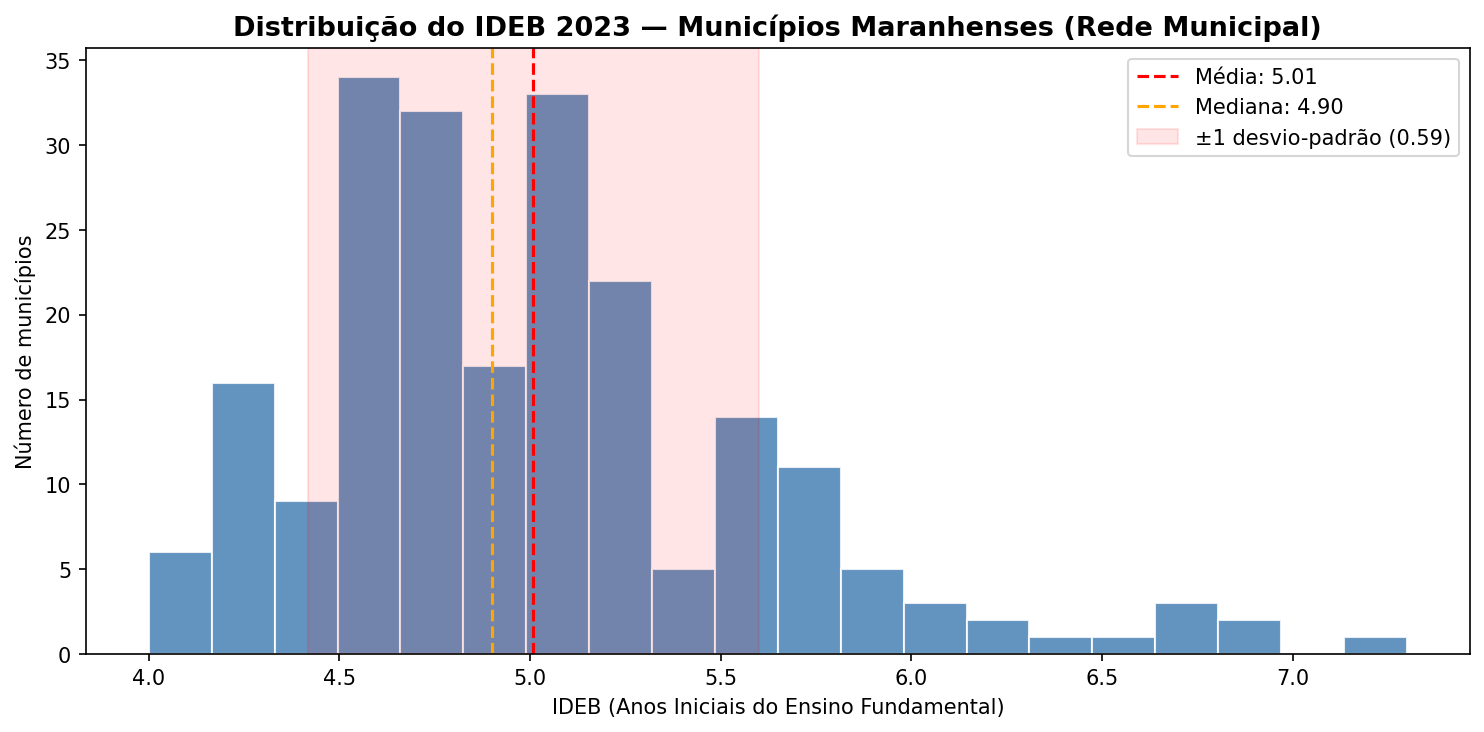
\includegraphics[width=0.85\textwidth]{distribuicao_ideb.png}
  \caption{Distribuição do IDEB 2023, municípios maranhenses, rede municipal, Anos Iniciais do EF. Linha vermelha tracejada: média (5,01); linha laranja tracejada: mediana (4,90); faixa vermelha: intervalo $\pm 1$ desvio-padrão.}
  \label{fig:dist_ideb}
\end{figure}

A amplitude de 3,30 pontos (4,00 a 7,30) é expressiva dado que o IDEB varia de 0 a 10. Isso indica que, mesmo dentro do Maranhão (estado homogeneamente vulnerável em termos nacionais) existe variabilidade interna substancial que justifica investigar os fatores associados aos destaques positivos.

Os percentuais médios das variáveis de infraestrutura revelam disparidades: a \textit{conectividade à internet} está presente em 73,7\% das escolas municipais do cluster vulnerável e em 81,9\% das escolas do cluster de maior renda; já o acesso a \textit{biblioteca ou sala de leitura} é notavelmente baixo em ambos os grupos (12,5\% nas escolas vulneráveis), sugerindo que esse recurso pode ser um diferencial relevante justamente por sua raridade. A proporção média de \textit{docentes EFAI com ensino superior} é de 60,5\% nos municípios mais vulneráveis e de 73,9\% naqueles de maior renda, diferença que antecipa uma das hipóteses testadas no estágio intragrupo.

\section{Modelagem}

\subsection{Seleção do Número de Clusters}

A Figura~\ref{fig:elbow} apresenta as curvas de inércia (cotovelo) e Silhouette Score para $k \in \{2, \ldots, 10\}$. O Silhouette Score atinge seu valor máximo em $k = 2$ (0,619), indicando dois grupos bem separados no espaço {renda, IDHM}. O Método do Cotovelo confirma a escolha: a queda marginal de inércia entre $k = 2$ e $k = 3$ é consideravelmente menor que entre $k = 1$ e $k = 2$. A estabilidade bootstrap (ARI médio = 0,89 em 25 iterações) confirma que a partição é robusta.

\begin{figure}[H]
  \centering
  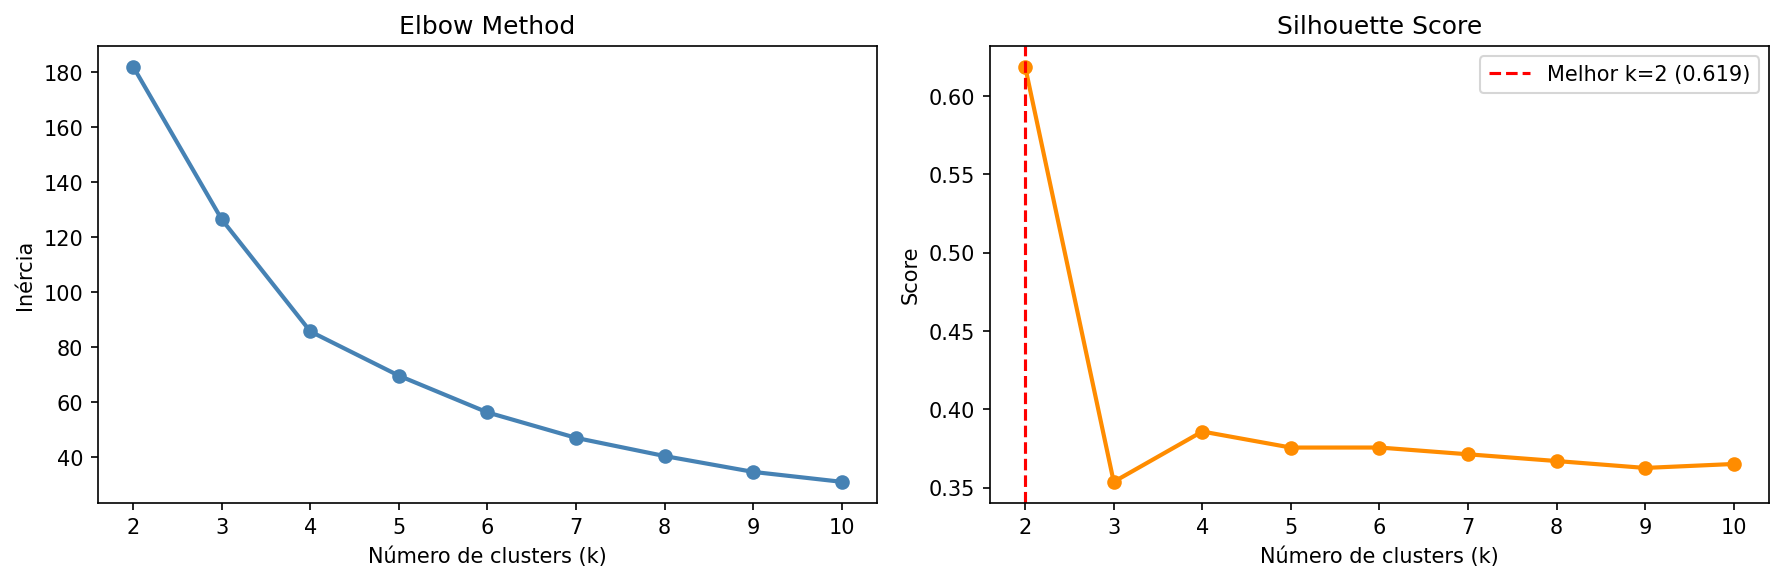
\includegraphics[width=0.90\textwidth]{elbow_silhouette.png}
  \caption{Curvas de inércia (esquerda) e Silhouette Score (direita) para $k \in \{2, \ldots, 10\}$. A linha vertical vermelha indica o $k$ ótimo segundo o silhouette.}
  \label{fig:elbow}
\end{figure}

\subsection{Estrutura dos Clusters}

A Figura~\ref{fig:pca} exibe os clusters projetados nas duas primeiras componentes principais (PC1 explica 88,4\% da variância; PC2 explica 11,6\%). A separação visual entre os dois grupos é clara, confirmando a coerência da partição.

\begin{figure}[H]
  \centering
  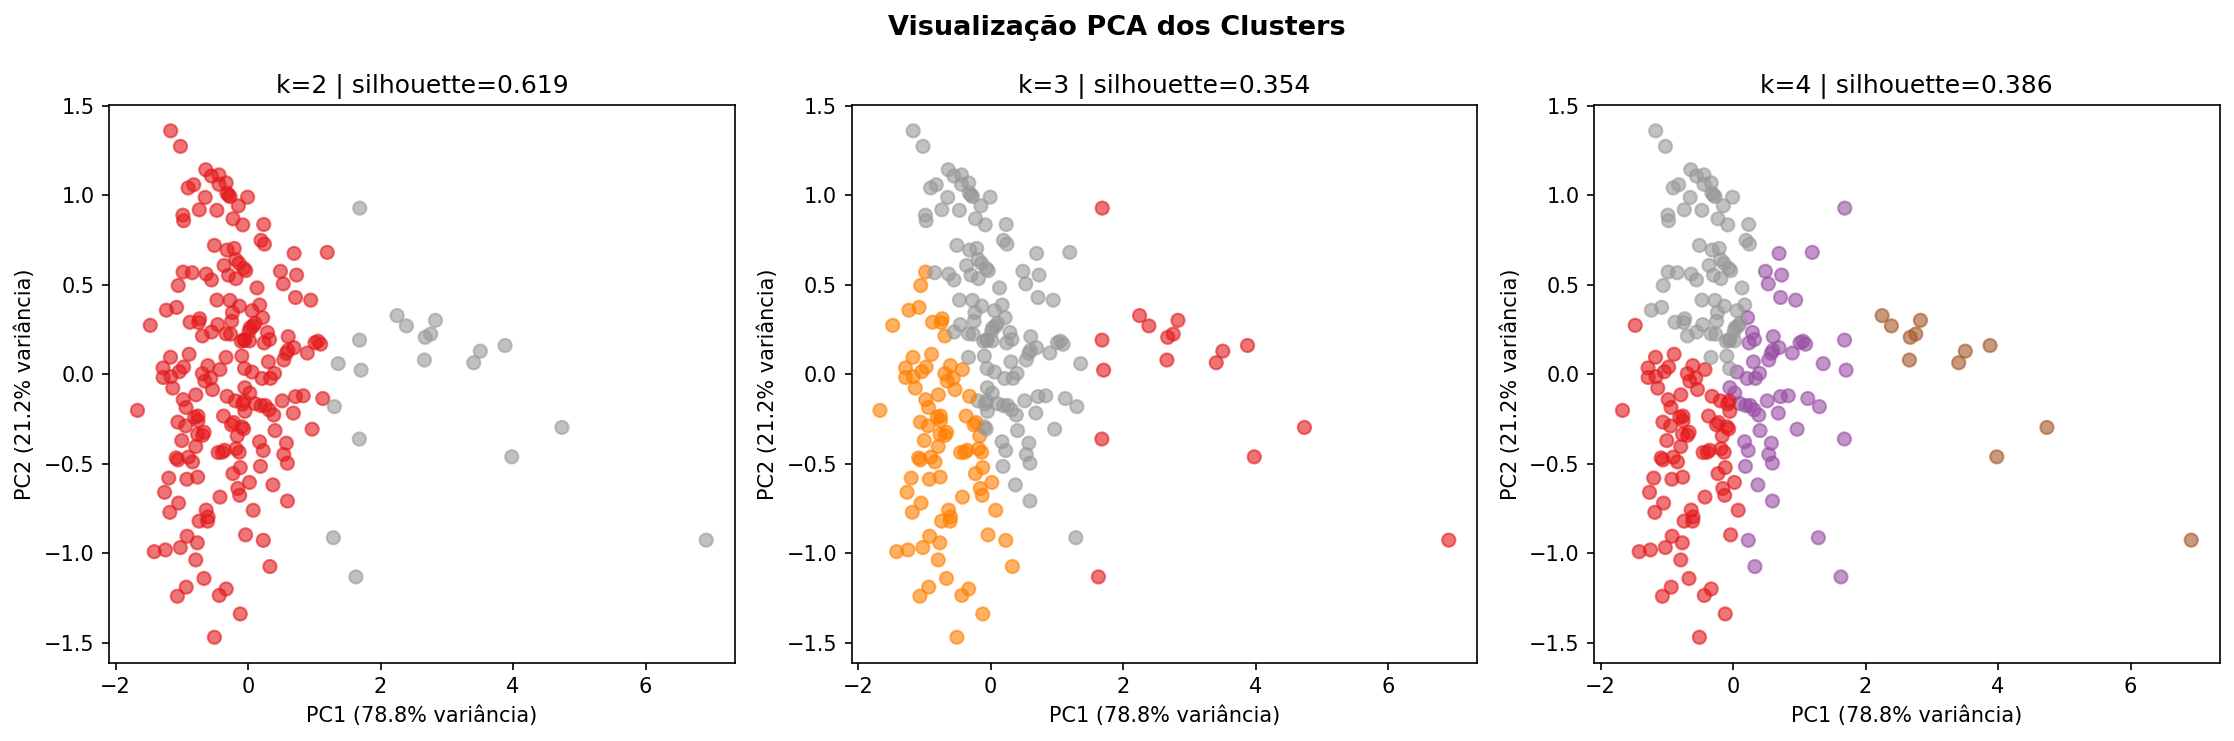
\includegraphics[width=0.85\textwidth]{pca_clusters.png}
  \caption{Visualização PCA dos clusters de municípios maranhenses para $k \in \{2, 3, 4\}$. A separação em dois grupos é a mais nítida.}
  \label{fig:pca}
\end{figure}

Os dois clusters obtidos são denominados pelo critério de renda média:

\begin{itemize}
  \item \textbf{Cluster ``vulneráveis''} (n = 197): renda per capita média de R\$ 210, IDHM médio de 0,737, IDEB médio de 4,96.
  \item \textbf{Cluster ``maior renda''} (n = 20): renda per capita média de R\$ 447, IDHM médio de 0,780, IDEB médio de 5,45. Inclui municípios como Açailândia, Balsas, Bacabal e Alto Parnaíba.
\end{itemize}

O cluster de maior renda conta com apenas 20 municípios, número insuficiente para a análise intragrupo por quantis (que requereria ao menos 20 observações em cada subgrupo extremo). A análise comparativa detalhada é portanto conduzida exclusivamente no cluster vulnerável.

\section{Resultados e Discussão}

\subsection{Fatores Discriminantes no Cluster Vulnerável}

Dentro do cluster vulnerável (n = 197), os 50 municípios do quartil superior de IDEB (alto, $\geq 5{,}20$, média 5,65) são comparados aos 50 do quartil inferior (baixo, $\leq 4{,}50$, média 4,35). A diferença média de 1,30 ponto de IDEB entre os grupos é substancial: equivale a mais de dois desvios-padrão da distribuição estadual.

A Figura~\ref{fig:rf_vulneraveis} apresenta as importâncias do Random Forest Classifier para o cluster vulnerável. As oito variáveis de maior importância são, em ordem decrescente: \textit{renda per capita} (0,121), \textit{média de alunos por turma no EF básico} (0,098), \textit{\% escolas com biblioteca/sala de leitura} (0,096), \textit{\% docentes com ensino superior} (0,093), \textit{proxy de distorção idade-série} (0,090), \textit{\% docentes com licenciatura} (0,087), \textit{média de alunos por turma no EF anos finais} (0,074) e \textit{\% escolas com esgoto adequado} (0,073).

\begin{figure}[H]
  \centering
  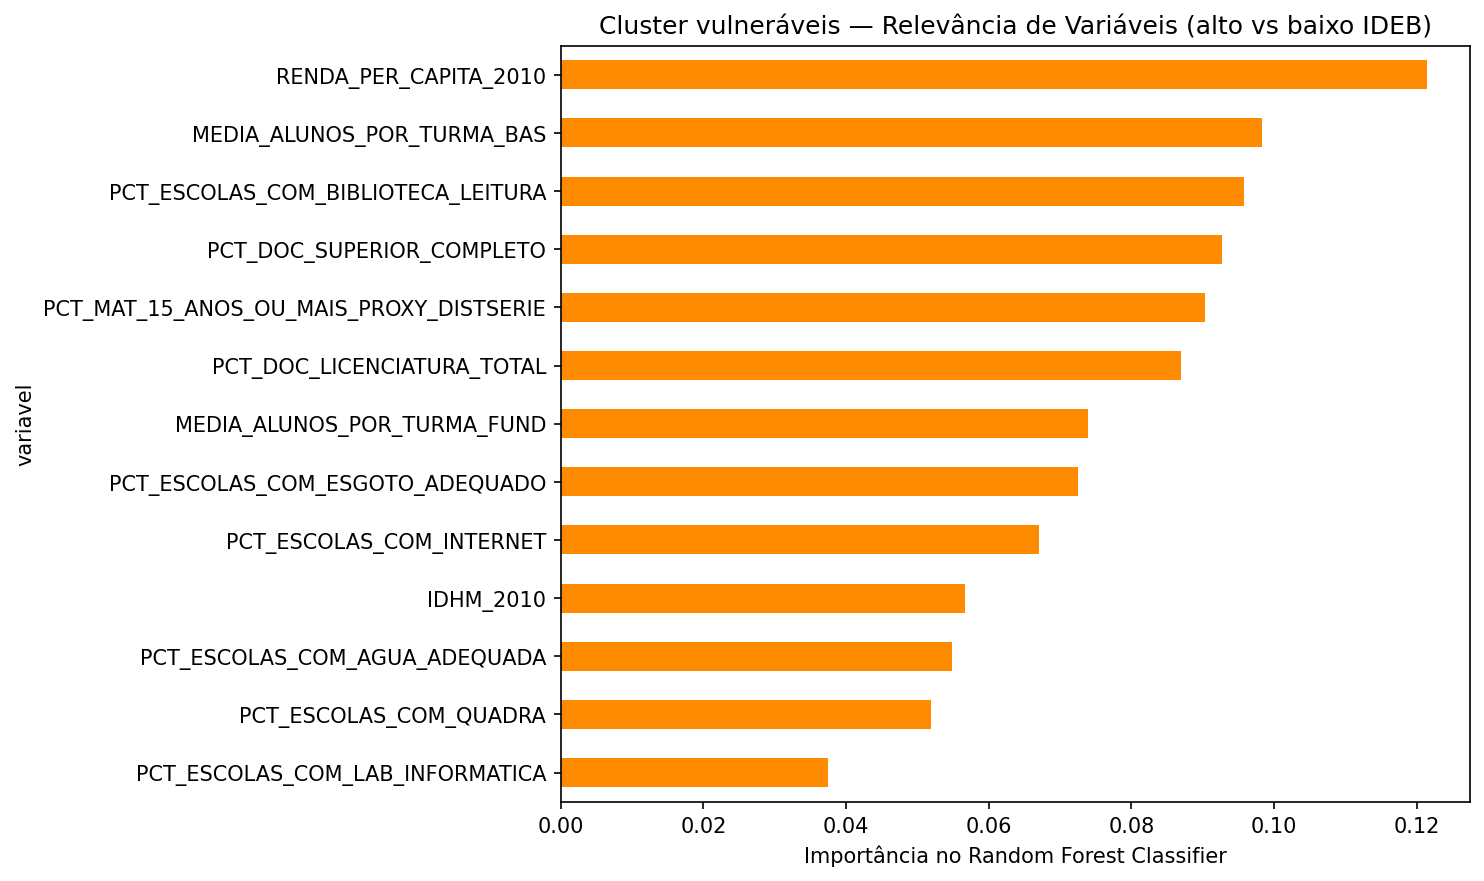
\includegraphics[width=0.85\textwidth]{cluster_vulneraveis_variaveis_relevantes_destaque.png}
  \caption{Importâncias do Random Forest Classifier para diferenciar municípios de alto e baixo IDEB no cluster vulnerável.}
  \label{fig:rf_vulneraveis}
\end{figure}

O Teste de Mann-Whitney complementa a análise ao indicar quais variáveis apresentam diferenças estatisticamente significativas entre os grupos. A Tabela~\ref{tab:mw} resume os resultados para as variáveis com $p < 0{,}10$.

\begin{table}[H]
\centering
\caption{Variáveis com diferença significativa entre municípios de alto e baixo IDEB, Cluster vulnerável (Mann-Whitney bicaudal)}
\label{tab:mw}
\begin{tabular}{lcccc}
\toprule
\textbf{Variável} & \textbf{Média alto} & \textbf{Média baixo} & \textbf{$\Delta$} & \textbf{p-valor} \\
\midrule
\textit{\% doc. com licenciatura}     & 68,0\% & 59,4\% & +8,6 p.p. & 0,023** \\
\textit{\% doc. com ensino superior}  & 66,8\% & 58,5\% & +8,3 p.p. & 0,026** \\
\textit{\% escolas com biblioteca}    & 13,8\% & 10,5\% & +3,3 p.p. & 0,030** \\
\textit{\% escolas com internet}      & 77,1\% & 69,5\% & +7,6 p.p. & 0,062*  \\
\textit{Alunos/turma EF (média)}      & 22,9   & 21,9   & +1,0      & 0,066*  \\
\bottomrule
\multicolumn{5}{l}{\footnotesize Sig.: ** $p < 0{,}05$; * $p < 0{,}10$.}
\end{tabular}
\end{table}

A formação docente emerge como o fator intracontextual mais consistentemente associado ao desempenho superior: municípios vulneráveis de alto IDEB têm, em média, 8,5 p.p. a mais de \textit{docentes com ensino superior} e 8,6 p.p. a mais com \textit{licenciatura} em comparação aos de baixo IDEB. Esse achado é convergente com a literatura internacional. \citet{rivkin2005} demonstraram que a qualidade do professor é o fator intraescolar de maior impacto sobre o aprendizado. Estudos nacionais também apontam formação docente como variável central nos resultados do IDEB \cite{vasconcelos2021}.

O acesso a \textit{biblioteca ou sala de leitura}, ainda que presente em apenas 10--14\% das escolas, também aparece como fator discriminante ($p = 0{,}030$). Sua raridade torna essa variável um alvo direto de intervenção: pequenas expansões na proporção de escolas com espaços de leitura estruturados podem fazer diferença mensurável no IDEB municipal.

A \textit{conectividade à internet} ($p = 0{,}062$) e o \textit{tamanho médio de turma} ($p = 0{,}066$) são significativos ao nível de 10\%, sinalizando tendências relevantes para políticas, embora com menor robustez estatística dada a variabilidade intragrupo.

A \textit{renda per capita} aparece com a maior importância no Random Forest (0,121) mesmo dentro do cluster vulnerável, onde a variação de renda é estruturalmente menor. Isso sugere que, mesmo após a segmentação socioeconômica, a heterogeneidade residual de renda dentro do grupo tem poder preditivo, o que reforça a importância de controles socioeconômicos em análises educacionais, mesmo dentro de grupos nominalmente homogêneos.

\section{Implicações Práticas}

Os resultados têm implicações diretas para gestores municipais e formuladores de políticas educacionais do Maranhão. Três direções de ação emergem dos achados:
\begin{itemize}
  \item \textbf{Formação e habilitação docente.} A diferença de 8,5 p.p. na proporção de \textit{docentes com ensino superior} entre municípios de alto e baixo IDEB, dentro do mesmo contexto socioeconômico, indica que programas de formação continuada e de indução à licenciatura específica têm potencial de impacto real sobre o IDEB. Políticas estaduais e federais de financiamento de graduação a distância para docentes em exercício (como o Programa Nacional de Formação de Professores da Educação Básica --- Parfor) são alvos naturais de expansão nos municípios do cluster vulnerável.

  \item \textbf{Espaços de leitura nas escolas.} A escassez de \textit{bibliotecas e salas de leitura} (presentes em apenas 10--14\% das escolas) e sua associação significativa com desempenho superior sugerem que investimentos relativamente modestos em acervo e espaço físico podem ser custo-efetivos. Municípios com IDEB baixo dentro do cluster vulnerável têm, em média, 3,3 p.p. menos escolas com esse recurso.

  \item \textbf{Conectividade digital.} A diferença de 7,6 p.p. na proporção de \textit{escolas com internet} aponta para o efeito mediado da conectividade sobre o IDEB: embora o impacto seja apenas marginalmente significativo ($p = 0{,}062$), a convergência com a importância no Random Forest justifica o monitoramento desse indicador como parte de estratégias de melhoria educacional.
\end{itemize}
\chapter{Conclusions}
\label{cap:conclusions}

\section{Comparison with IDEB Works}


\section{Limitations and Future Direction}
\section{Acknowledgments}


\section{Authors' CRediT}

\bibliographystyle{abntex2-alf}
\bibliography{references}

\end{document}